\documentclass[12pt,a4paper]{article}
\usepackage[utf8]{inputenc}
\usepackage[ngerman]{babel}
\usepackage{amsmath}
\usepackage{amsfonts}
\usepackage{amssymb}
\usepackage{graphicx}
\usepackage{pdfpages}
\usepackage{titling}
\usepackage{float}
\usepackage[format=plain,
      justification=RaggedRight,
      singlelinecheck=false]
     {caption}
\usepackage[left=2.5cm,right=2.5cm,top=2.5cm,bottom=3cm]{geometry}
\author{Janik Frick}
\title{Konzipierung und Erstellung eines Parametertabellenkonfigurators und Praxisnahe Mitarbeit im releasten Produkt LC-VISION}
\usepackage{setspace}
\usepackage{scrextend}
\deffootnote[1em]{1em}{1em}{%
   \textsuperscript{\thefootnotemark}%
}

\usepackage{fancyhdr}
\addtolength{\headheight}{1.5cm} % make more space for the header
\pagestyle{fancyplain} % use fancy for all pages except chapter start
\lhead{
\includegraphics[width=50mm,scale=1]{blum-logo.PNG}}
\rhead{
\includegraphics[width=50mm,scale=1]{dhbw.png}}
\renewcommand{\headrulewidth}{0pt} % remove rule below header

\newcommand{\dualerPartner}{Blum-Novotest GmbH, Standort Grünkraut}
\newcommand{\hochschule}{Dualen Hochschule Baden-Württemberg Ravensburg}
\newcommand{\betreuer}{Mallmann, Guilherme, Dr.-Ing.}
\newcommand{\studiengang}{Informatik}
\newcommand{\kurs}{TIT21, Matrikelnummer 4268671}
\pagenumbering{arabic}

\begin{document}
\begin{titlepage}

\includegraphics[width=50mm,scale=1]{blum-logo.PNG}
\hfill

\includegraphics[width=50mm,scale=1]{dhbw.png}
   \begin{center}
       \textbf{\huge{\thetitle}}\\
       \vspace{2.2cm}
       \Large{Projektarbeit T1000\\
       des Studiengangs \studiengang\\
       an der \hochschule\\
       \vspace{1.5cm}
       von\\
       \vspace{0.5cm}
       \theauthor}
       
   \end{center}
       \vspace{1.6cm}
       \noindent
       \vspace{0.3cm}
       \textbf{\large{Kurs: \kurs}}\\
       \vspace{0.3cm}
       \textbf{\large{Dualer Partner: \dualerPartner}}\\
       \vspace{0.3cm}
       \textbf{\large{Betreuer: \betreuer}}
       

\end{titlepage}
\onehalfspacing
\tableofcontents
\newpage
\section{Einleitung}
Die Blum-Novotest GmbH(Blum) ist im Bereich Maschinenbau für Mess- und Prüftechnik tätig. Am Standort Grünkraut (Baden-Württemberg) ist der Hauptsitz der Firma. Dort befinden sich Entwicklung und Fertigung für den Bereich Messtechnik. Am zweiten Standort in Willich (Nordrhein-Westfalen) sind die Entwicklung und Fertigung im Bereich Prüftechnik untergebracht.\\
Produkte von Blum werden in vielen anspruchsvollen Industrien im Bereich der Qualitätssicherung eingesetzt. Die Kunden kommen unter anderem aus der Automobil-, Luftfahrt- und der Werkzeugmaschinenindustrie. \\
An die Produkte dieser Industrien werden höchste Ansprüche in Sachen Qualität gestellt. Daraus resultieren auch für die Produkte der Firma Blum höchste Ansprüche. \\
Um diese Ansprüche erfüllen zu können, werden sowohl bestehende Produkte laufend optimiert und weiterentwickelt, als auch neue Produkte entwickelt. \\
Die Arbeit wird im Umfeld von Blum am Standort Grünkraut verfasst. \\
Ziel der Arbeit ist es die vielfältigen Aspekte der Softwareentwicklung kennenzulernen und den Einstieg zu schaffen.\\
Um dieses Ziel zu erreichen, besteht der praktische Teil aus zwei Projekten.\\
Mit der Entwicklung eines \glqq Parametertabellenkonfigurators\grqq\space sollen die verschiedenen Aufgaben der Softwareentwicklung veranschaulicht werden.\\
Durch die Mitarbeit am schon bestehenden Produkt \glqq LC-Vision\grqq\space wird die Produktpflege und Weiterentwicklung thematisiert. 
Außerdem wird dabei das Einarbeiten in unbekannten Code relevant, was ein wichtiger Bestandteil der Produktpflege ist.
\newpage   
\section{Softwareentwicklung}
Softwareentwicklung besteht nicht nur aus dem Schreiben von Software. Auch die Entwicklung von Software ist ein Projekt. Man beginnt mit dem Sammeln der Anforderungen, startet die Entwicklung von Prototypen und geht in die Implementierung. Der Prozess endet mit der Produktpflege und dem Service.  
\subsection{Anforderungsanalyse}
Eindeutige und präzise Anforderungen bilden die Grundlage für ein funktionierendes Projekt\cite{doi:10.1080/12460125.2016.1187390}. \\
Daraus folgt, dass es nicht ausreichend ist, die Liste der Anforderungen zu lesen. Anforderungen müssen analysiert und mit weiterem Wissen über das Projektumfeld kombiniert werden. \\
Dafür gibt es mehrere Techniken, die eingesetzt werden können. 
\subsubsection{Interviews}
\label{interview}
Interviews bieten die Möglichkeit in direkten Gesprächen mit Personen aus dem Umfeld des Projekts Informationen zu sammeln. Diese Informationen können Risiken sein, die zu berücksichtigen sind, Schwierigkeiten bei der aktuellen Vorgehensweise, sowie Abläufe die beibehalten werden sollten. \\
Der Erfolg dieser Vorgehensweise hängt dabei von allen Beteiligten Personen ab. Fehlt Wissen über das Umfeld des Projekts kann es zu Schwierigkeiten beim Sammeln der Fragen kommen, wodurch manche Aspekte nicht berücksichtigt werden. Auch die Befragten können Probleme haben ihre Gedanken und ihr Wissen wiederzugeben\cite{tiwari2012selecting}. Das kann die Auswertung der Antworten erschweren.
\subsubsection{Fragebögen}
\label{Fragebögen}
Fragebögen geben den Befragten Personen die Möglichkeit ohne direkte Beeinflussung durch den Ersteller der Fragen, Informationen bereitzustellen. Zusätzlich reduzieren sie den Zeitdruck unter dem geantwortet werden soll und alle Befragten antworten auf die gleiche Fragestellung.\\
Fragebögen können eingesetzt werden um Annahmen zu bestätigen oder nach Meinungen und Vorschlägen zu fragen\cite{tiwari2012selecting}. \\
Bei Einsatz dieser Methode ist darauf zu achten die Fragen offen zu formulieren, um die Antworten nicht in eine Richtung zu lenken. 
\subsubsection{Beobachtung}
\label{Beobachtung}
Die Beobachtungsmethode dient dazu aus beobachteten Vorgängen Informationen zu sammeln. \\
Diese Beobachtung kann offen oder verdeckt durchgeführt werden. Bei der verdeckten Vorgehensweise ist das beobachtete Verhalten natürlicher und realistischer, als bei der offenen Vorgehensweise\cite{silhavy2011requirements}. \\
Mit diesem Vorgehen lassen sich Abläufe bei Aufgaben nachvollziehen. Gründe für dieses Abläufe sollten durch andere Techniken in Erfahrung gebracht werden.\\
\subsubsection{Anforderungstypen}
\label{Anforderungstypen}
Anforderungen können in zwei Typen unterteilt werden: Die funktionalen und die nicht funktionalen Anforderungen.
\\Funktionale Anforderungen geben vor, für welche Aufgaben das Produkt geplant wird und welche Funktionen dafür benötigt werden. Die Validierung dieser Anforderungen ist gegeben, da am Ende eindeutig ist, ob eine Funktionalität verfügbar ist. \\
Die nicht funktionalen Anforderungen geben vor, mit welchem Vorgehen und welchen Tools eine Funktion umgesetzt werden soll\cite{10.1145/2884781.2884788}. \\
Nicht funktionale Anforderungen sind häufig unpräzise formuliert und somit problematisch in der Validierung\cite{10.1145/2884781.2884788}.
\subsection{Dokumentation}
\label{Dokumenation}
Die Dokumentation von Softwareprojekten ist neben der eigentlichen Entwicklung ein relevanter Teilaspekt. Die Dokumentation dient zur Sicherung von Wissen und Grundlagen von Entscheidungen. \\
Die Dokumentation kann in zwei Bereiche unterteilt werden. Die Dokumentation der Software und die Dokumentation für den Anwender\cite{THEUNISSEN2022106733}.\\
\underline{Software-Dokumentation}\\
Diese Form der Dokumentation soll Wissen über die Software beinhalten. Dazu zählen Grundlagen für Entscheidungen der Softwarearchitektur und die Aufgaben von Funktionen, Methoden und Variablen.\\
Die Relevanz besteht darin Wissensverlust zu verhindern, der entsteht, wenn der Entwickler nicht zur Verfügung steht. Dieser Verlust beeinflusst die Einarbeitungsdauer eines neuen Mitarbeiters und somit auch die Produktpflege. \\
Diese Problematik der mangelnden Softwaredokumentation ist in agilen Umfeldern bekannt. Sich ändernde Anforderungen verursachen die Notwendigkeit die Software anzupassen, was Anpassungen der Dokumentation erfordert. Geänderte Anforderungen bringen auch neue kurzfristige Aufgaben mit sich, denen eine höhere Priorität beigemessen wird, als der Aktualisierung der Dokumentation. Kommen viele Änderungen in kurzer Zeit stauen sich die anstehenden Änderungen auf und sorgen für einen hohen Zeitaufwand der Dokumentation. Dies resultiert oftmals in einer vernachlässigten Dokumentation.\\
Weitere potentielle Schwierigkeiten resultieren aus der Ansicht, dass der Code bereits eine ausreichende Dokumentation für diesen Zweck darstellt und dass Informationen häufig informell und verbal kommuniziert werden, was dazu führen kann, dass diese Informationen nach der Verarbeitung nirgends festgehalten sind und dadurch verloren gehen können\cite{THEUNISSEN2022106733}.\\

\underline{User-Dokumentation}\\
Der Dokumentation für die Anwender und die Betreuer wird meist mehr Bedeutung beigemessen, da sie für den Einsatz des Produktes relevant ist.\\
Diese Dokumentation beinhaltet Fehlermeldungen, Voraussetzungen für die Installation und Informationen für die Verwendung. Probleme mit dieser Dokumentation können Schwierigkeiten im Kundenservice verursachen. Da Probleme dieser Art einen direkten Einfluss auf den Erfolg eines Produktes oder der Firma haben können. Diese möglichen Konsequenzen sorgen dafür, dass dieser Dokumentation mehr Bedeutung beigemessen wird\cite{THEUNISSEN2022106733}.

\subsection{Grobentwurf}
Beim Grobentwurf werden die Hauptbestandteile der Software und die Softwarearchitektur geplant. Dabei sollte der Kunde möglichst miteinbezogen werden, denn der Kunde hat großen Anteil am Gelingen des Projekts\cite{10.1145/1060710.1060712}. \\
Um den Kunden einzubeziehen können Prototypen eingesetzt werden.\\
Hat das Programm eine Graphische Benutzeroberfläche(GUI) so kann der Grobentwurf unterschiedlich geplant werden. \\
\subsubsection{GUI mit Bildern}
\label{GUI mit Bildern}
Der Grobentwurf der GUI kann mit Hilfe von Bildern in einem beliebigen Bilderstellungsprogramm nachgebildet werden. Die erstellten Entwürfe dienen als Gesprächsgrundlage für eventuell notwendige Veränderungen. Hierbei ist zu beachten, dass die Simulation von Verbindungen zwischen GUI-Elementen zeitaufwendig oder gar nicht möglich ist.
\subsubsection{Prototypen}
\label{Prototypen}
Ein Prototyp ist eine funktionierende, begrenzte Version der Anwendung, die als Basis für Gespräche und die Entwicklung weiterer Prototypen dient\cite{budde1992prototyping}. \\
Dieser Prototyp kann durch Software, oder mit einem Mockup-Tool\footnote{Tool um ein GUI zu simulieren}, oder auch in einer Software für Präsentationen, realisiert werden. Ein Software basierter Prototyp erfordert die Mitarbeit der Entwickler im Design Prozess. 
\subsubsection{User-Tests}
\label{User-Tests}
Bei User Tests wird einer oder mehreren Testpersonen, abhängig von der Verfügbarkeit, der aktuelle Prototyp \ref{Prototypen} vorgelegt. Dann kann man der Testperson eine konkrete Aufgabe geben, oder sie den Prototyp frei entdecken lassen. Bei beiden Vorgehensweisen werden Probleme dokumentiert. Hat man mehrere Testpersonen zur Verfügung können auch Gruppentests durchgeführt werden. Bei diesen arbeiten mehrere Personen an einer Aufgabe. Bei Einzel-Tests lassen sich Probleme im Ablauf besser erkennen. In Gruppen-Tests hingegen werden die tatsächlichen Probleme der Testpersonen besser erkenntlich.\cite{BASTIEN2010e18}. \\
Mit dieser Testmethodik lassen sich nur Prototypen \ref{Prototypen} testen, da nur hier die Verbindungen funktional sind.
\subsubsection{30-Sekunden Tests}
\label{30-Sekunden Tests}
Bei 30-Sekunden-Tests bekommen die Testpersonen 30 Sekunden Zeit um den Prototyp zu erkunden. Nach 30 Sekunden wird ein Fragebogen ausgefüllt, auf dem die Übersichtlichkeit bewertet wird\cite{vsimek2015usability}. \\
30-Sekunden Tests lassen sich mit Bildentwürfen \ref{GUI mit Bildern} und mit Prototypen \ref{Prototypen} durchführen, da es bei beiden Entwürfen möglich ist ein Element für 30 Sekunden zu zeigen.
\subsubsection{Heatmaps}
\label{Heatmaps}
Heatmaptools markieren farbig welche Bereiche einer Benutzeroberfläche oft genutzt werden und welche seltene\cite{10.1145/2470654.2466442}. Diese Daten geben Informationen darüber ob Kernfunktionen anders positioniert werden sollten.\\
Diese Methode lässt sich für Bildentwürfe \ref{GUI mit Bildern} und Prototypen \ref{Prototypen} verwenden.

\subsection{Implementierung}
In der Implementierung ist der Aufwand abhängig von der Vorgehensweise. Wird das GUI mit Hilfe von Bildentwürfen \ref{GUI mit Bildern} entwickelt, ist der Aufwand der Implementierung höher, da die Applikation von Grund auf programmiert werden muss. \\
Wird mit Prototypen \ref{Prototypen} gearbeitet, ist die Implementierung weniger aufwendig. Kommt ein Mockup-Tool zum Einsatz muss die Software ebenfalls von Grund auf programmiert werden, aber der Mock-Up Prototyp dient als Hilfestellung um die Übersicht über die notwendigen Verbindungen zwischen GUI Elementen zu behalten.\\
Ist der Prototyp programmiert werden, ist die Struktur fertig und muss gegebenenfalls um Funktionen ergänzt werden, die im Grobentwurf nicht berücksichtigt wurden. \\
Entscheidungen was Design und Technologien betrifft, sollten vor Beginn der Implementierung getroffen worden sein. Die Aufgabe der Entwickler besteht darin das geplante Design so in Module zu unterteilen, das es programmiert werden kann\cite{rakos1990software}. 
\subsubsection{Tests}
\label{Tests}
Durch Tests wird validiert, ob die Software die Anforderungen erfüllt. Dabei sollten alle Ergebnisse von Tests dokumentiert werden, um Fehlerquellen, Lösungen und die Kosten für das Beheben der Fehler im Überblick zu behalten\cite{rakos1990software}.\\
Diese bestehen aus mehreren Stufen.\\
\underline{Modultests}\\
Programmierte Module werden isoliert getestet, um zu prüfen, ob das Modul die Aufgaben erfüllt. Dazu kann auch ein simulierter Input verwenden, wenn benötigte Module noch nicht verfügbar sind. \\
Diese Tests können in zwei Arten unterteilt werden. Bei 'white-box' Tests wird das Modul in einzelnen Schritten getestet. Der Tester weiß wie die Daten verarbeitet werden. Bei 'black-box' Tests versucht der Tester das Vorgehen eines Nutzers nachzustellen. Dabei ist dem Tester die genaue Verarbeitung egal\cite{rakos1990software}.\\
\underline{Low-Level Integrationstests}\\
In diesem Stadium werden die Aufrufe und Rückgabewerte von anderen Modulen getestet. Dabei spielt es keine Rolle, von wem die abhängigen Module entwickelt wurden. Stehen keine realen Daten zur Verfügung kann mit simulierten Daten gearbeitet werden.\cite{rakos1990software}.\\
Ob diese Tests manuell oder automatisiert stattfinden hängt von unterschiedlichen Faktoren ab.\\
\newline
Mit diesem Vorgehen sind alle Module und ihre Abhängigkeiten auf ihre Funktionalität überprüft. Auf dieser Basis wird eine Version erstellt und getestet die in dieser Form praxistauglich ist. Parallel wird daran gearbeitet die benötigten Umgebungsbedingungen bereitzustellen. Dieses Setup wird auf Funktionalität geprüft. Bei erfolgreichem Verlauf der Tests kann die Dokumentation \ref{Dokumenation} fertiggestellt werden.
Bestätigt der Kunde das Resultat kann mit dem Training betreuender Personen und Benutzern begonnen werden\cite{rakos1990software}.\\
\subsubsection{Test Automatisierung}
Das manuelle Ausführen von Tests kann zeitaufwändig sein, wodurch man auf die Idee kommen kann diese Tests zu automatisieren. Diese Entscheidung ist dabei von unterschiedlichen Faktoren abhängig. \\
Die Erfahrung des Verantwortlichen beeinflusst die Dauer für die Automatisierung maßgeblich. Auch die Umgebung in der die Anwendung funktionieren soll, muss automatisiert simuliert werden. Basiert die Funktionalität der Software auf Benutzereingaben, oder läuft sie nach dem Start alleine? Anwendungen die selbstständig ablaufen, sind meistens einfacher zu testen, als solche bei denen man eine automatisierte Benutzerinteraktion nachstellen muss\cite{fewster1999software}. 
\subsection{Objektorientierung}
\label{Objektorientierung}
\section{Parametertabellenkonfigurator}
Mit Hilfe des \glqq Parametertabellenkonfigurators\grqq\space sollen die Abläufe der Konfiguration unterstützt werden.
\subsection{Problemstellung}
Bei bestehenden Programmen für numerische Steuerungen müssen während der Inbetriebnahme Parametertabellen in einem beliebigen Texteditor angepasst werden. Aufgrund der Anzahl, wie auch der Einstellmöglichkeiten der Parameter, wird hierfür eine separate Installationsanleitung benötigt. Der Prozess der Parametrierung ist daher Fehleranfällig und von der Erfahrung des Inbetriebnehmers abhängig. Um den hohen Anforderungen der Kunden gerecht zu werden, gilt es potentielle Fehlerquellen zu eliminieren. Hierfür soll selbstständig ein \glqq Parametertabellenkonfigurator\grqq\space entwickelt werden.
\subsection{Anforderungen} 
An den \glqq Parametertabellenkonfigurator\grqq\space gibt es mehrere Anforderungen. \\
Parametertabellen sollen eingelesen und angezeigt werden können. Zu den Parametern soll es ermöglicht werden Beschreibungen aus Text und Bild speichern und anzeigen zu können.\\
Diese Anforderungen sind aus dem Bereich der funktionalen Anforderungsen \ref{Anforderungstypen}\\
Nicht funktionale Anforderungen \ref{Anforderungstypen} sind die Verwendung der Programmiersprache und das Verwenden des in C++ entwickelten Framework Qt.\\
Aus diesen Anforderungen lässt sich ableiten welche GUI-Elemente nötig sind und welche Funktionalitäten benötigt werden.\\
Um die Anforderungen an den \glqq Parametertabellenkonfigurator\grqq\space zu sammeln, die nicht im Auftragsdokument stehen, wurde das Interview \ref{interview} gewählt. Die Entscheidung wurde getroffen weil in offenen Gesprächen mehr Zusatzinformationen fließen, als in Umfragen \ref{Fragebögen} oder durch Beobachtung \ref{Beobachtung}. Zusätzlich kann auf Verständnisschwierigkeiten reagiert werden, solange das Gespräch noch aktuell ist und der Kontext noch nicht vergessen ist.\\
Hauptergebnis ist die Bedeutung eines übersichtlichen GUI.
\subsubsection{Notwendige Funktionalitäten}
Um die Parametertabellen anzeigen zu können müssen diese aus einer Datei eingelesen werden. Um Konfigurationen festzuhalten wird eine Funktion zum Speichern der Tabellen benötigt. \\
Für die Beschreibungen wird zusätzlich eine Funktion benötigt um diese mit den richtigen Parametern zu verknüpfen. \\
\subsubsection{Notwendige GUI-Elemente}
Das GUI benötigt Anzeigemöglichkeiten für die Parametertabellen und Beschreibungen, Angaben von Namen, Steuerung und Produkttyp zur aktuellen Parametertabelle und den aktuellen Parameter.\\
Benötigte Steuerelemente sind Möglichkeiten um Parametertabellen und Beschreibungen szu laden und zu speichern. 
\subsection{GUI-Entwurf}
Um das GUI zu entwerfen kommt ein Prototyp \ref{Prototypen} zum Einsatz, der mit dem Mockup-Tool "Balsamiq Mockup 3" erstellt wurde. Das Tool bietet nahezu alle gängigen GUI-Elemente an und kann diese miteinander verknüpfen, so dass schon in einem frühen Stadium die Funktionalität gegeben ist und besprochen werden kann. Zusätzlich bietet das Tool eine unkomplizierte Möglichkeit alternative Entwürfe zu entwerfen und in den Ablauf der Simulation zu integrieren. Das unterstützt den Prozess während der Entwicklung des GUI, da neue Vorschläge in kurzer Zeit besprochen und weiterentwickelt werden können.\\
\newline
Das GUI ist aus mehreren einzelnen Fenstern aufgebaut. Dieser Aufbau unterstützt die Übersichtlichkeit und der Benutzerführung bei der Verwendung, da jeweils nur die benötigten Informationen und Funktionen angezeigt werden.\\ 
Insgesamt besteht das GUI aus vier Fenstern die dem Benutzer die benötigten Funktionen zur Verfügung stellen. \\
Ein Fenster dient dem Zweck bei erster Benutzung den Pfad zu einer Datenbank, in der die Beschreibungen gespeichert sind, einzugeben. Im nächsten Fenster lässt sich die Auswahl der Parametertabellen konfigurieren. Nach der Auswahl einer Parametertabelle wird diese im Hauptfenster angezeigt. In diesem Fenster werden die Beschreibungen der Parameter angezeigt und die Parametertabelle kann angepasst werden. Es gibt Steuerelemente für die Navigation durch die Parametertabelle, für die Navigation durch die Fenster und die Möglichkeit die geänderte Parametertabelle zu speichern.\\
\begin{figure}[H]
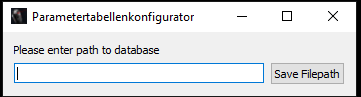
\includegraphics[scale=1]{pictures_and_research/Bilder/filepathWindow.PNG}
\caption{Fenster um den Dateipfad der Datenbank einzugeben,\\
es gibt einen Standardpfad}
\end{figure}
\begin{figure}[H]
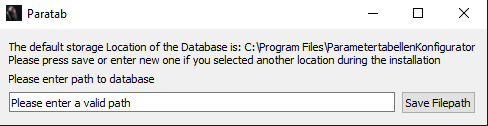
\includegraphics[scale=1]{pictures_and_research/Bilder/errorFilePathW.PNG}
\caption{Wurde ein nicht vorhandener Pfad eingegeben erscheint die Fehlermeldung "Please enter a valid path"}
\end{figure}
\begin{figure}[H]
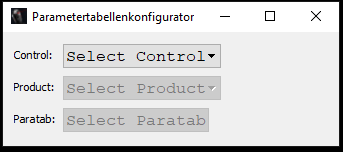
\includegraphics[scale=1]{pictures_and_research/Bilder/configW.PNG}
\caption{Fenster um Auswahl der Parametertabellen zu konfigurieren}
\end{figure}
\begin{figure}[H]
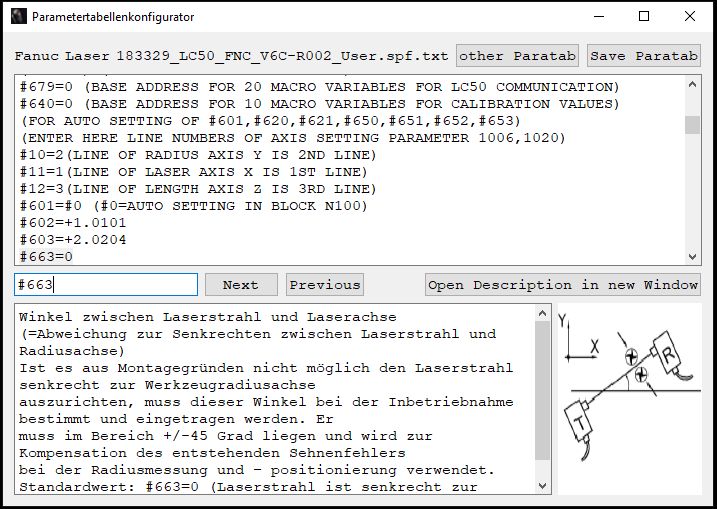
\includegraphics[scale=0.75]{pictures_and_research/Bilder/paratabW.PNG}
\caption{Fenster für die Anzeige der Parametertabellen und deren Beschreibungen}
\end{figure}
\noindent
In Abbildung 4 werden im Oberen Bereich werden Informationen zur aktuell ausgewählten Parametertabelle angezeigt. Oben rechts gibt es Steuerelemente um eine andere Parametertabelle auszuwählen, oder die Aktuelle zu speichern.\\
Unterhalb der Anzeige für die Parametertabelle ist der Bereich für detaillierte Informationen zum aktuellen Parameter. Es gibt Steuerelemente um andere Parameter auszuwählen. Dies ist mit den Buttons "Next" und "Previous" möglich, die jeweils um einen Parameter nach oben oder nach unten springen. Durch direkte Eingabe eines Parameters in das Parameterfeld kann zu einem beliebigen Parameter gesprungen werden. Um größere Beschreibungen übersichtlich sehen zu können gibt es die Möglichkeit die Beschreibung isoliert in einem neuen Fenster zu öffnen.\\
\begin{figure}[H]
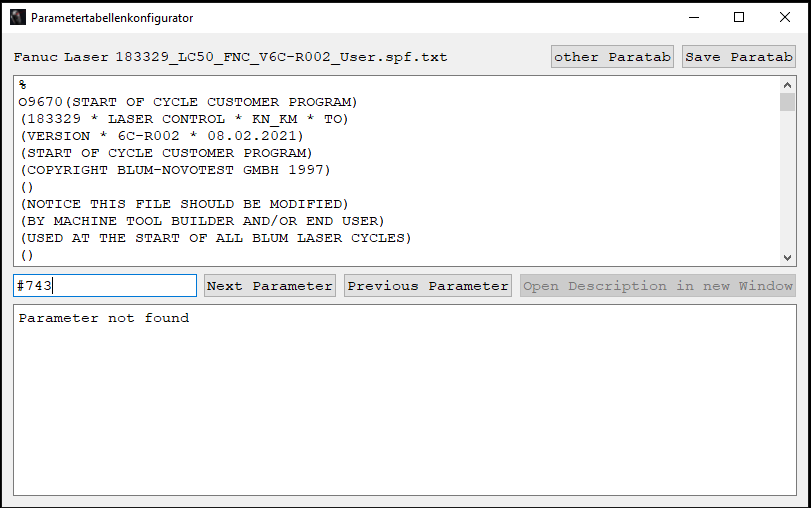
\includegraphics[scale=0.6]{pictures_and_research/Bilder/fehlermeldung_invalid_parameter.PNG}
\caption{Wird ein nicht vorhandener Parameter in das Feld eingegeben wird eine Fehlermeldung angezeigt.}
\end{figure}
\begin{figure}[H]
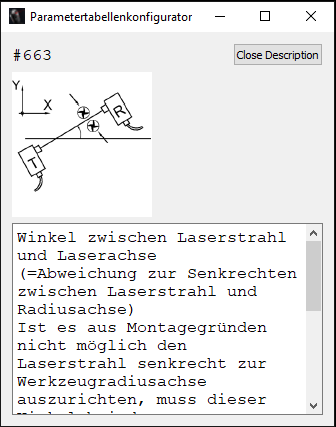
\includegraphics[scale=1]{pictures_and_research/Bilder/descriptW.PNG}
\caption{Isolierte Ansicht einer Beschreibung eines Parameters}
\end{figure}\noindent
Das in Abbildung 6 sichtbare Bild hat eine konstante Größe. Der Grund dafür ist dass ansonsten bei Änderung der Fenstergröße das Bild verzerrt werden würde und das Erkennen von wichtigen Informationen im Bild erschwert werden würde.
\subsection{Programmierung}
Für die Programmierung des \glqq Parametertabellenkonfigurator\grqq\space kommt das für GUI optimierte C++ Framework Qt zum Einsatz. \\
\subsubsection{Softwarestruktur}
Für die Programmierung kommt die objektorientierte Programmierung \ref{Objektorientierung} zum Einsatz, da sich Elemente eines GUI gut als Objekt darstellen lassen.
Die Software ist modular aufgebaut. Das bedeutet sie besteht aus einzelnen Modulen, die jeweils eine bestimmte Aufgabe übernehmen. Um die Module miteinander zu verknüpfen gibt es Klassen, die für die Aufrufe der entsprechenden Module verantwortlich sind. \\
Dieses Design bietet die Möglichkeit die Anzeige der Daten von der grundlegenden Logik getrennt zu verwalten.\\
Die Module haben vorgegebene Schnittstellen, die von den \lq Managerklassen\rq\space bedient werden. Diese Schnittstellen rufen die internen Methoden des Moduls auf. Somit lässt sich der Inhalt und die Funktionsweise eines Moduls verändern ohne dass der Aufruf des Interface durch die \lq Managerklassen\rq\space verändert werden muss. Dadurch entsteht eine hohe Flexibilität. \\
\begin{figure}[H]
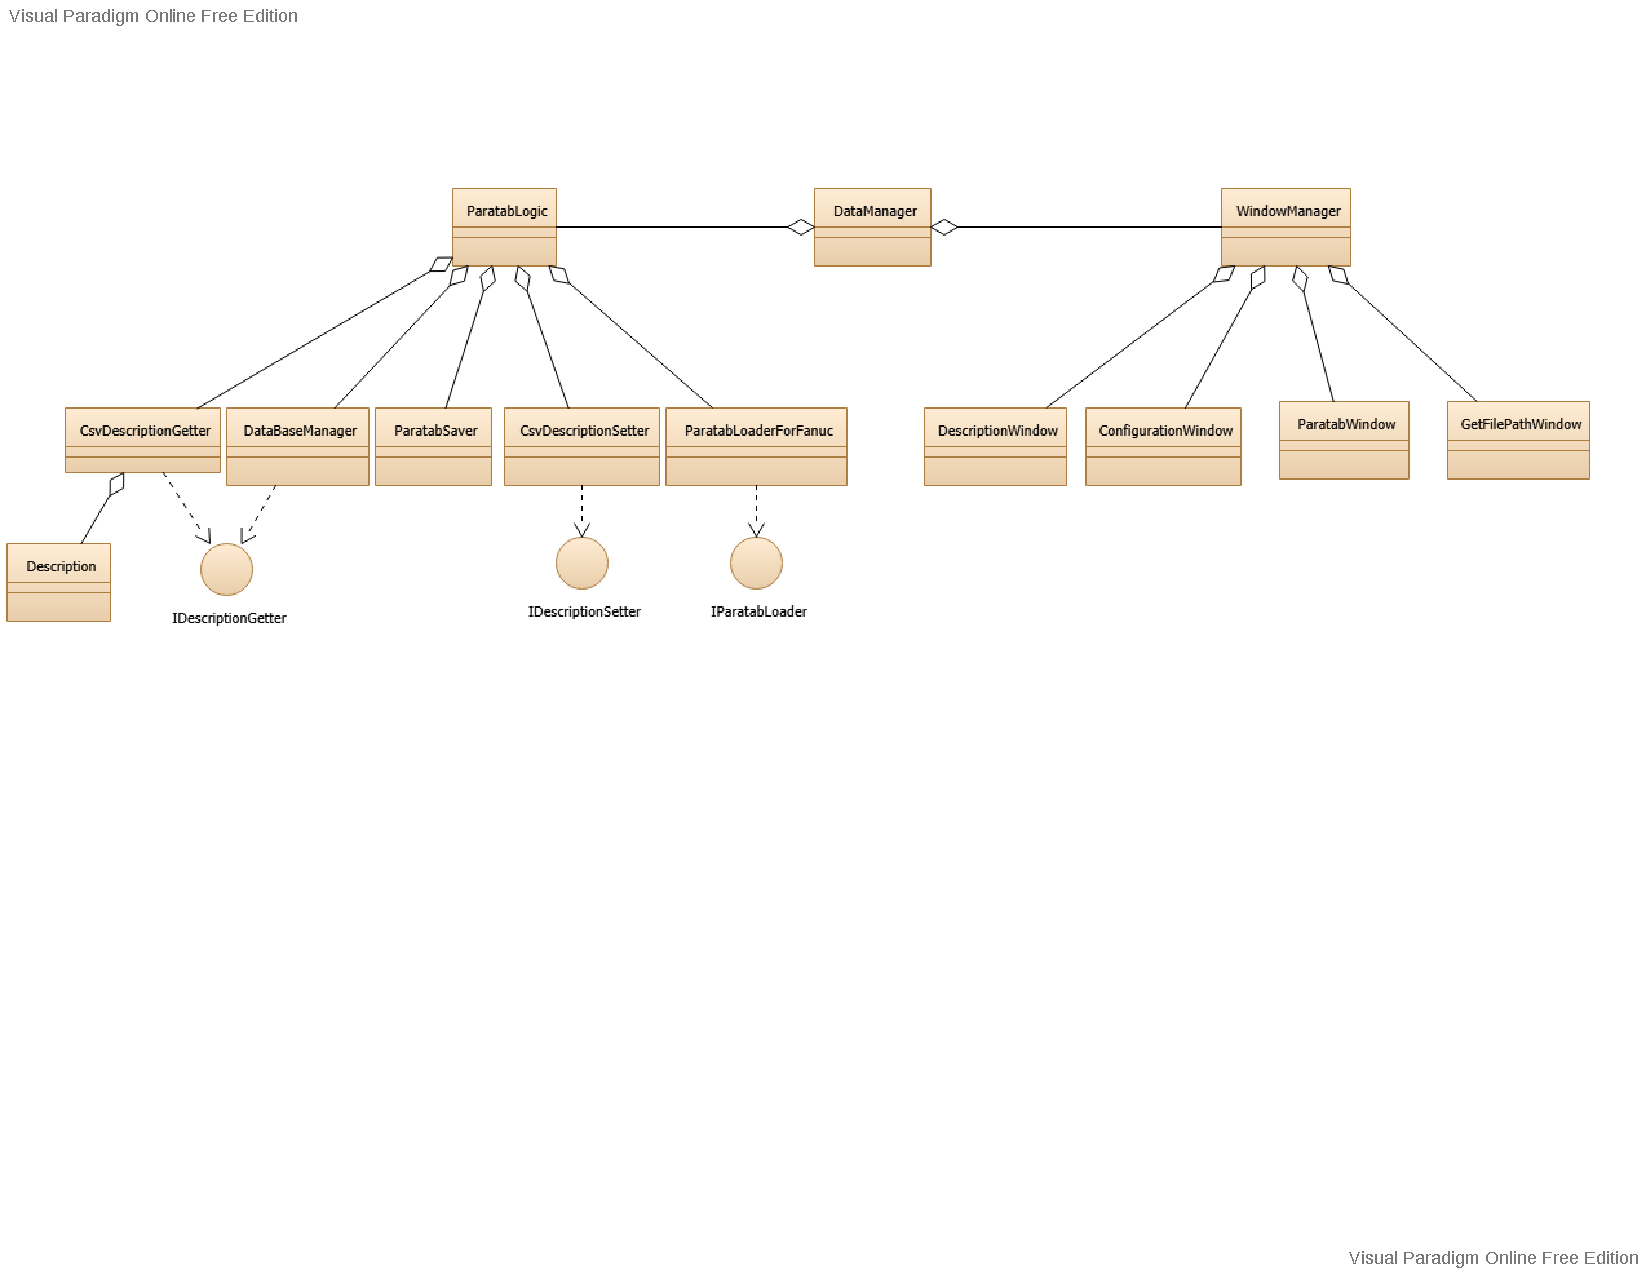
\includegraphics[page=1,scale=0.6]{pictures_and_research/pdf_files/smallParatabUml.pdf}
\caption{UML-Diagramm der Software ohne Inhalte der Klassen}
\end{figure}
Das in Abbildung 7 dargestellte Diagramm dient zur Veranschaulichung der Modularität der Software, aus Gründen der Übersichtlichkeit wurde daher auf den Inhalt der einzelnen Klassen verzichtet.
\subsubsection{•}
\section{LC-Vision}
\newpage

\newpage
\bibliography{references, tandf_tjds2025_302}
\bibliographystyle{ieeetr}
\end{document}<div class="open_grepper_editor" title="Edit & Save To Grepper"></div>
